% Ludwik Ciechański
\documentclass[12pt]{article}
    
\usepackage[T1]{fontenc}
\usepackage{beramono}
\usepackage{polski}
\usepackage[utf8]{inputenc}
\usepackage[a4paper, total={6in, 10in}]{geometry}
\usepackage{listings}
\usepackage[usenames,dvipsnames]{xcolor}
\usepackage{graphicx}
\usepackage{float}
\usepackage{color}
\usepackage{titlesec}
\usepackage[hidelinks]{hyperref}
\usepackage[font=small]{caption}

\newcommand{\cFaculty}[1]{\Large \textsc{#1}\par}
\newcommand{\cSubject}[1]{\Large #1\par}
\newcommand{\cTitle}[1]{\LARGE \textbf{#1}\par}
\newcommand{\cAuthors}[1]{\large #1\par}
\newcommand{\cDate}[1]{\small #1\par}

\setcounter{section}{-1}
\setcounter{figure}{-1}
\graphicspath{ {images/} }
\titlespacing{\section}{0pt}{2pt}{2pt}
\titlespacing{\subsection}{0pt}{3pt}{2pt}

%%
%% Julia definition (c) 2014 Jubobs
%%
\lstdefinelanguage{Julia}
  {morekeywords={abstract,break,case,catch,const,continue,do,else,elseif,
      end,export,false,for,function,immutable,import,importall,if,in,
      macro,module,otherwise,quote,return,switch,true,try,type,typealias,
      using,while},
   sensitive=true,
   alsoother={$},
   morecomment=[l]\#,
   morecomment=[n]{\#=}{=\#},
   morestring=[s]{"}{"},
   morestring=[m]{'}{'},
}[keywords,comments,strings]

\lstset{
  language         = Julia,
  basicstyle       = \fontsize{10}{12}\selectfont\ttfamily,
  keywordstyle     = \bfseries\color{blue},
  stringstyle      = \color{magenta},
  commentstyle     = \color{ForestGreen},
  showstringspaces = false,
  aboveskip=3mm,
  belowskip=3mm,
  numbers=none,
  breaklines=true,
  breakatwhitespace=true,
  tabsize=4,
  frame=shadowbox
}


\begin{document}

% strona tytułowa
\noindent%
\begin{minipage}[t]{.35\textwidth}
    \vspace{0pt}
    
\includegraphics[scale=0.36]{logoAGH}
\end{minipage}%
\begin{minipage}[t]{.65\textwidth}
    \vspace{2pt}
    \cFaculty{Katedra Informatyki}
    \cSubject{Metody obliczeniowe w nauce i technice}
    \vspace{10pt}
    \cTitle{Laboratorium 6 - interpolacja\\ sprawozdanie z ćwiczenia}
    \vspace{10pt}
    \cAuthors{Ludwik Ciechański}
    \cDate{\today}
\end{minipage}
\vspace{30pt}

% --------------------
\section{\bf Przygotowanie}

\subsection{\bf używane pakiety}
\begin{lstlisting}
using Plots
using Polynomials
using DataFrames
using Statistics
using Interpolations
\end{lstlisting}

\subsection{\bf przykładowe dane}
\begin{lstlisting}
# wylosowanie wezlow interpolacji
xs = 1:1:10
A = [rand() for x in xs]
# geste punkty do rysowania wykresow funkcji interpolujacych
xsf = 1:0.02:10
\end{lstlisting}

\subsection{\bf ilustracja}
\begin{center}
    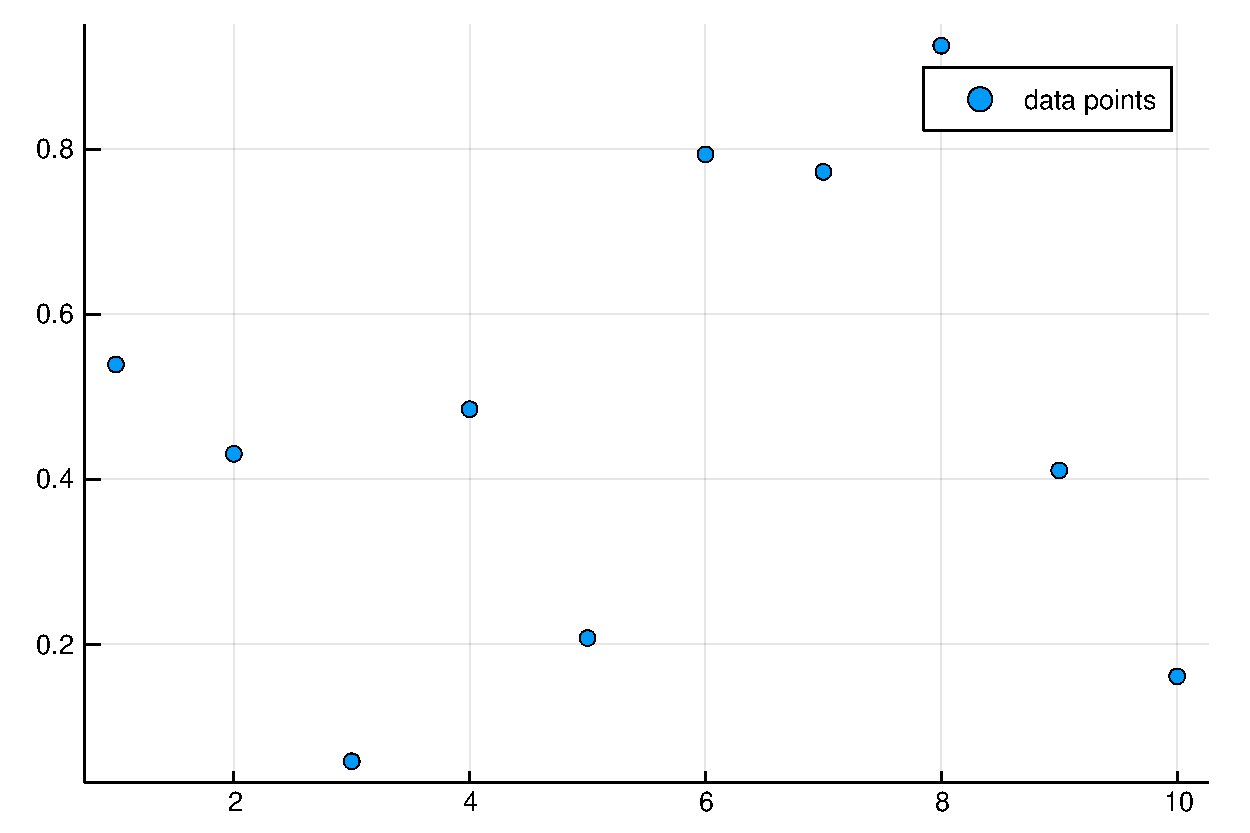
\includegraphics[width=0.87\textwidth]{plot0.pdf}
\end{center}
\clearpage
% ----------------------------------
\section{\bf Wielomian interpolacyjny Lagrange’a}

\subsection{\bf wzory}
    . . .

\subsection{\bf kod}
\begin{lstlisting}
function lagrange_interpolation(xs, A)   
    n = size(A,1)
    P = Poly([0])
    for k = 1:n
        l = Poly([1.0])
        for i = 1:n
            if i != k
                l = l * poly([xs[i]]) / (xs[k] - xs[i])
            end
        end            
        P += (l * A[k])
    end
    P
end
\end{lstlisting}
\begin{lstlisting}
fit1 = lagrange_interpolation(xs, A)
B1 = [fit1(x) for x in xsf]
p1 = scatter(xs, A, label="data points")
plot!(xsf, B1, label="lagrange interpolation")
savefig(p1, "img/plot1.pdf")
\end{lstlisting}

\subsection{\bf wykres}
\begin{center}
    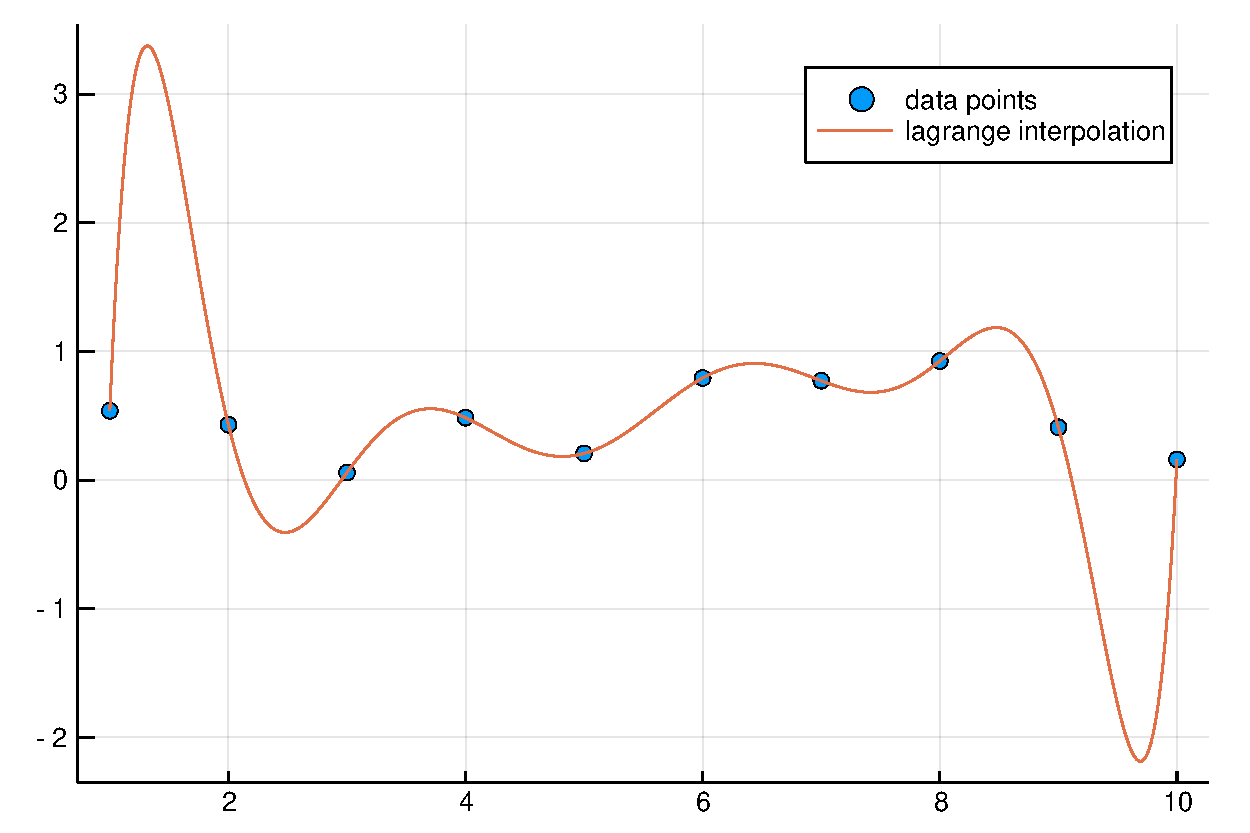
\includegraphics[width=0.95\textwidth]{plot1.pdf}
    \captionof{figure}{Interpolacja wielomianem Lagrange'a}
\end{center}
\clearpage
% ----------------------------------
\section{\bf Metoda Newtona (ilorazów róznicowych)}

\subsection{\bf wzory}
    . . .

\subsection{\bf kod}
\begin{lstlisting}
function newton_interpolation(xs, A, n)
    if n == 1
        Poly(float(A[1]))
    else
        prev = newton_interpolation(xs, A, n-1)
        p = A[n] - polyval(prev, xs[n])
        q = 1
        for i = 1:n-1
            q = q * (xs[n] - xs[i])
        end        
        poly([xs[i] for i in 1:n-1]) * (p / q) + prev
    end
end
\end{lstlisting}
\begin{lstlisting}
fit2 = newton_interpolation(xs, A, size(A,1))
B2 = [fit2(x) for x in xsf]
p2 = scatter(xs, A, label="data points")
plot!(xsf, B2, color=:orange, label="newton interpolation")
savefig(p2, "img/plot2.pdf")
\end{lstlisting}

\subsection{\bf wykres}
\begin{center}
    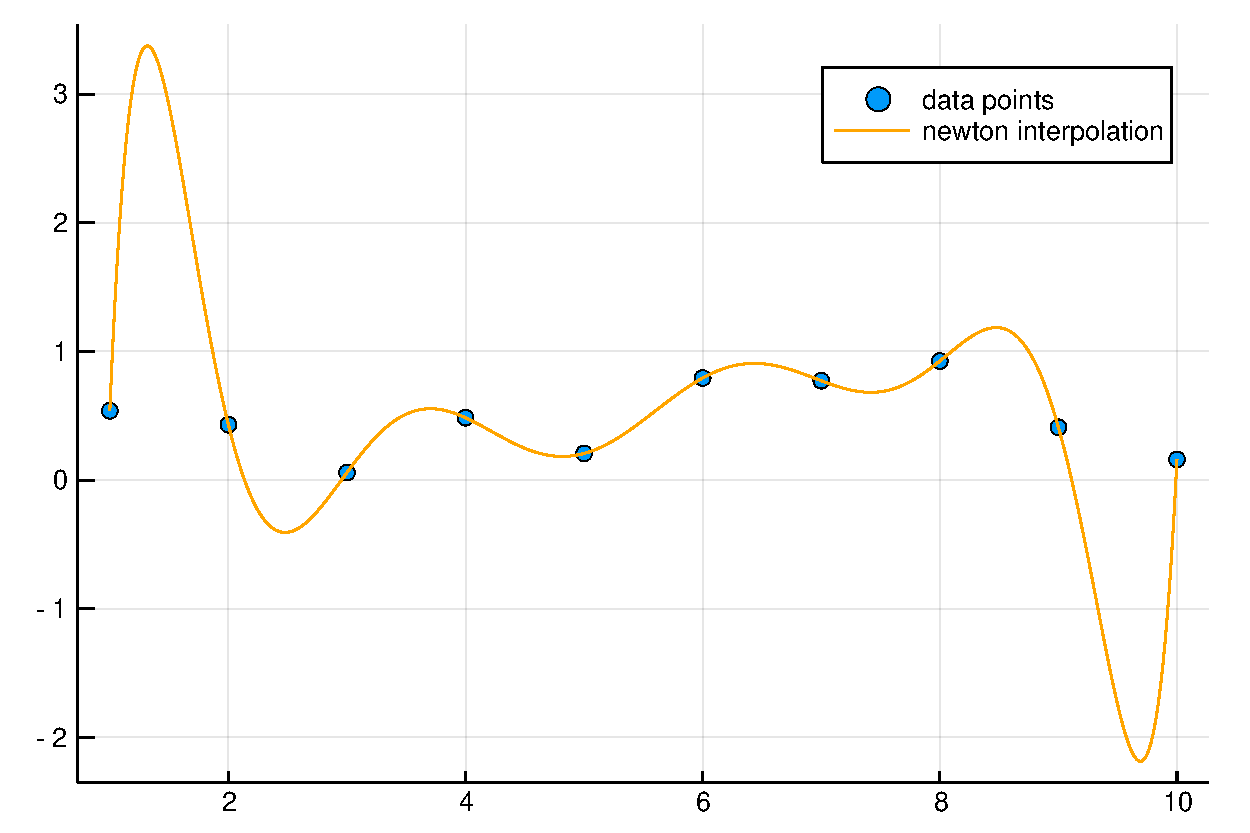
\includegraphics[width=0.97\textwidth]{plot2.pdf}
    \captionof{figure}{Interpolacja metodą Newtona}
\end{center}
\clearpage
% ----------------------------------

% spis tresci
\tableofcontents

\end{document}